\documentclass[12pt,letterpaper]{article}
\usepackage{graphicx,textcomp}
\usepackage{natbib}
\usepackage{setspace}
\usepackage{fullpage}
\usepackage{color}
\usepackage[reqno]{amsmath}
\usepackage{amsthm}
\usepackage{fancyvrb}
\usepackage{amssymb,enumerate}
\usepackage[all]{xy}
\usepackage{endnotes}
\usepackage{lscape}
\newtheorem{com}{Comment}
\usepackage{float}
\usepackage{hyperref}
\newtheorem{lem} {Lemma}
\newtheorem{prop}{Proposition}
\newtheorem{thm}{Theorem}
\newtheorem{defn}{Definition}
\newtheorem{cor}{Corollary}
\newtheorem{obs}{Observation}
\usepackage[compact]{titlesec}
\usepackage{dcolumn}
\usepackage{tikz}
\usetikzlibrary{arrows}
\usepackage{multirow}
\usepackage{xcolor}
\newcolumntype{.}{D{.}{.}{-1}}
\newcolumntype{d}[1]{D{.}{.}{#1}}
\definecolor{light-gray}{gray}{0.65}
\usepackage{url}
\usepackage{listings}
\usepackage{color}

\graphicspath{ {./images/} }

\definecolor{codegreen}{rgb}{0,0.6,0}
\definecolor{codegray}{rgb}{0.5,0.5,0.5}
\definecolor{codepurple}{rgb}{0.58,0,0.82}
\definecolor{backcolour}{rgb}{0.95,0.95,0.92}

\lstdefinestyle{mystyle}{
	backgroundcolor=\color{backcolour},   
	commentstyle=\color{codegreen},
	keywordstyle=\color{magenta},
	numberstyle=\tiny\color{codegray},
	stringstyle=\color{codepurple},
	basicstyle=\footnotesize,
	breakatwhitespace=false,         
	breaklines=true,                 
	captionpos=b,                    
	keepspaces=true,                 
	numbers=left,                    
	numbersep=5pt,                  
	showspaces=false,                
	showstringspaces=false,
	showtabs=false,                  
	tabsize=2
}
\lstset{style=mystyle}
\newcommand{\Sref}[1]{Section~\ref{#1}}
\newtheorem{hyp}{Hypothesis}

\title{Problem Set 1}
\date{Due: October 1, 2023}
\author{V. Dringelyte}

\begin{document}
	\maketitle
	
	\section*{Instructions}
	\begin{itemize}
	\item Please show your work! You may lose points by simply writing in the answer. If the problem requires you to execute commands in \texttt{R}, please include the code you used to get your answers. Please also include the \texttt{.R} file that contains your code. If you are not sure if work needs to be shown for a particular problem, please ask.
\item Your homework should be submitted electronically on GitHub.
\item This problem set is due before 23:59 on Sunday October 1, 2023. No late assignments will be accepted.
\item Total available points for this homework is 80.
	\end{itemize}
	
	\vspace{1cm}
	\section*{Question 1 (40 points): Education}

A school counselor was curious about the average of IQ of the students in her school and took a random sample of 25 students' IQ scores. The following is the data set:\\
\vspace{.5cm}

\lstinputlisting[language=R, firstline=43, lastline=43]{PS01(VD17341481).R}  

\vspace{1cm}

\begin{enumerate}
	\item Find a 90\% confidence interval for the average student IQ in the school.\\
	
		To calculate the confidence interval when the confidence coefficient = .90, I first found the mean:
		
		\lstinputlisting[language=R, firstline=60, lastline=61]{PS01(VD17341481).R}  
		
		This returned a mean of 98.44
		
		Then, I found the standard deviation:
		
		\lstinputlisting[language=R, firstline=65, lastline=65]{PS01(VD17341481).R}
		Which returned a value of 13.09
		
		So I could find the standard error.
		\lstinputlisting[language=R, firstline=69, lastline=69]{PS01(VD17341481).R} 
		Value of 2.62 
		
		Then I found the t-score
 		\lstinputlisting[language=R, firstline=73, lastline=73]{PS01(VD17341481).R}  
		
		I could use this to find the upper bounds of confidence interval
		\lstinputlisting[language=R, firstline=77, lastline=77]{PS01(VD17341481).R}  
		
		And the lower bounds of confidence interval
		\lstinputlisting[language=R, firstline=81, lastline=81]{PS01(VD17341481).R} 
		 
		This showed that the 90\% confidence interval for the the average student IQ is 
		93.96-102.92
	
	\item Next, the school counselor was curious  whether  the average student IQ in her school is higher than the average IQ score (100) among all the schools in the country.\\ 
	
	\noindent Using the same sample, conduct the appropriate hypothesis test with $\alpha=0.05$.
	
		To find the answer to this, I used the 5 steps of a statistical significance test.
		
		\textbf{Step 1: Assumptions.}
		
		1. The national average is 100.
		\lstinputlisting[language=R, firstline=94, lastline=94]{PS01(VD17341481).R} 
		2. The national sample has a normal distribution and random sampling, so we will use a t-score.
		
		\textbf{Step 2: State hypothesis.}
		
		The average IQ of the students in this school is higher than the average IQ score among all the schools in the country. The null hypothesis, then, is that the average IQ in the school is lower or equal to the average of schools nationally.
		
		\textbf{Step 3: Calculate a test statistic.}
		To do this, I used the formula:
	\begin{center}
		\large	$t=\frac{(\bar{y}-\mu)}{se}$
	\end{center}

		\normalsize In R:
		\lstinputlisting[language=R, firstline=104, lastline=107]{PS01(VD17341481).R}
		
		or, a faster way
	
		\lstinputlisting[language=R, firstline=111, lastline=111]{PS01(VD17341481).R}
		
		t-statistic = -0.59574
		
		\textbf{Step 4: Calculate a P-value}
		
		\lstinputlisting[language=R, firstline=114, lastline=114]{PS01(VD17341481).R}
		
		P-value = 0.722
		
		\textbf{Step 5: Draw a conclusion}
		As the P-value is larger than 0.05, we fail to reject the null hypothesis. So, the average IQ in the school is less than or equal to the average of schools in the country.
		
		
		
\end{enumerate}

\newpage

	\section*{Question 2 (40 points): Political Economy}

\noindent Researchers are curious about what affects the amount of money communities spend on addressing homelessness. The following variables constitute our data set about social welfare expenditures in the USA. \\
\vspace{.5cm}


\begin{tabular}{r|l}
	\texttt{State} &\emph{50 states in US} \\
	\texttt{Y} & \emph{per capita expenditure on shelters/housing assistance in state}\\
	\texttt{X1} &\emph{per capita personal income in state} \\
	\texttt{X2} &  \emph{Number of residents per 100,000 that are "financially insecure" in state}\\
	\texttt{X3} &  \emph{Number of people per thousand residing in urban areas in state} \\
	\texttt{Region} &  \emph{1=Northeast, 2= North Central, 3= South, 4=West} \\
\end{tabular}

\vspace{.5cm}
\noindent Explore the \texttt{expenditure} data set and import data into \texttt{R}.
\vspace{.5cm}
\lstinputlisting[language=R, firstline=131, lastline=131]{PS01(VD17341481).R}  
\vspace{.5cm}
\begin{itemize}

\item
Please plot the relationships among \emph{Y}, \emph{X1}, \emph{X2}, and \emph{X3}? What are the correlations among them (you just need to describe the graph and the relationships among them)?

I used the code we learnt in coding camp to plot these graphs.
\begin{verbatim}
	ggplot(expenditure, aes(x, y))+
	geom_point() +
	theme_classic()
\end{verbatim}


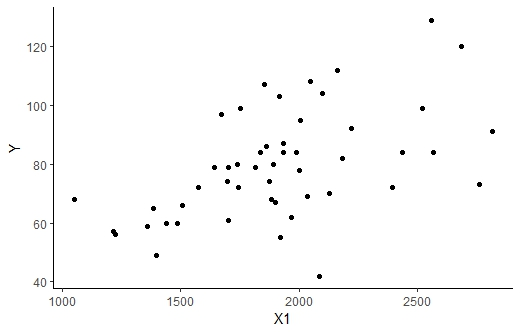
\includegraphics{YandX1}

\textbf{Y and X1.} There is a slight positive relationship between Y and X1, on the lower end, the relationship is stronger, and gets weaker as values increase.
\vspace{.5cm}

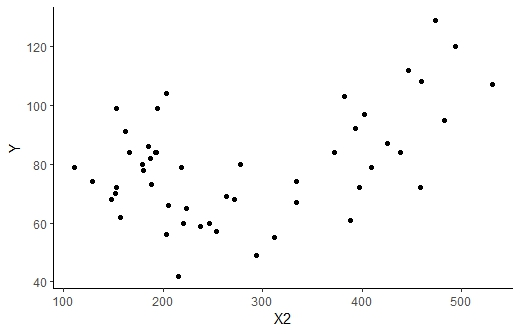
\includegraphics{YandX2}

\textbf{Y and X2.} The scatter plot forms a U shape. It seems that the relationship between Y and X2 is negative at first, but changes to a positive one near the middle of the graph.
\vspace{.5cm}

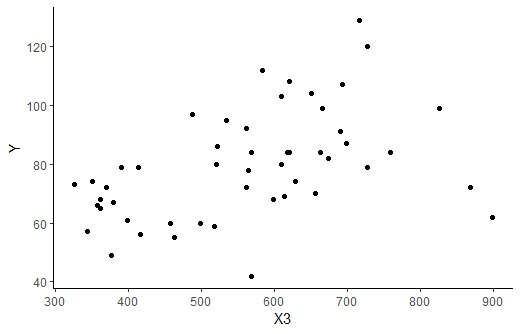
\includegraphics{YandX3}

\textbf{Y and X3.} There seems to be a slight positive relationship between Y and X3, as one increases, so does the other.
\vspace{.5cm}

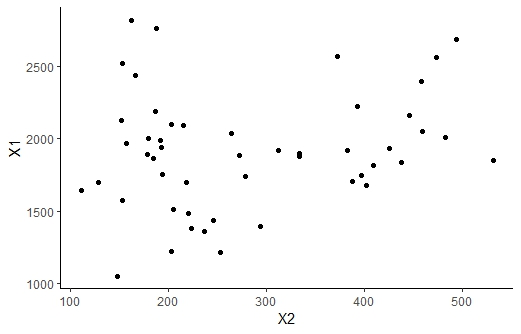
\includegraphics{X1andX2}

\textbf{X1 and X2.} The scatter plot forms a U shape. X2 values show little correlation to Y values.
\vspace{.5cm}

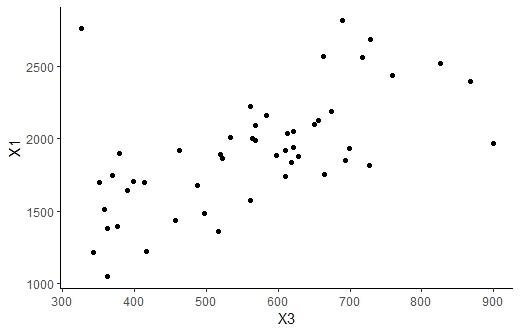
\includegraphics{X1andX3}

\textbf{X1 and X3.} There seems to be a positive relationship between X1 and X3 values. With the exception of some outliers, a lower X1 value correlates to a lower X3 value and vice versa.
\vspace{.5cm}

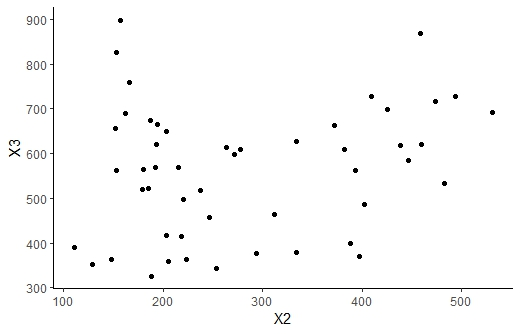
\includegraphics{X3andX2}

\textbf{X3 and X2.} The scatter plot shows a slight U shape. There seems to be very little correlation between X2 and X3.


\vspace{.5cm}
\item
Please plot the relationship between \emph{Y} and \emph{Region}? On average, which region has the highest per capita expenditure on housing assistance?

I thought the best way to show this relationship was using a box plot.

I used this code to plot this relationship:
\lstinputlisting[language=R, firstline=185, lastline=192]{PS01(VD17341481).R}
\newpage

Resulting in this box plot.

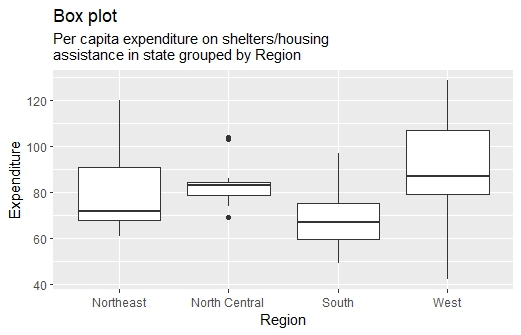
\includegraphics{RegionExBox}

In order to get the means, I had to take the four subsets out of the data, and turn them into separate objects:
\lstinputlisting[language=R, firstline=196, lastline=199]{PS01(VD17341481).R}
I used the code we learnt in coding camp for this.

Then, I found their respective means:
\lstinputlisting[language=R, firstline=202, lastline=205]{PS01(VD17341481).R}

This showed the following means:

\textbf{North-East:} 79.44

\textbf{North-Central:} 83.92

\textbf{South:} 69.19

\textbf{West:} 88.31

\newpage
I used this script to plot a new box plot:
\lstinputlisting[language=R, firstline=214, lastline=222]{PS01(VD17341481).R}

I came upon the issue that R saw the values for region as continuous, so I had to use the code \texttt{x = factor} to ensure that these values were categorical when plotting the graph. And I also used the code \texttt{ stat\_summary(fun.y="mean", color="red")} to show the means. I adapted this from  \href{https://www.geeksforgeeks.org/how-to-show-mean-value-in-boxplots-with-ggplot2/}{code I found online}.

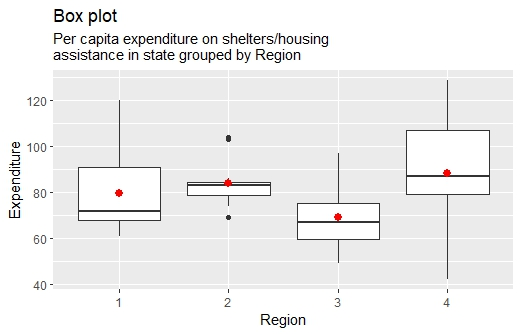
\includegraphics{RegionEx}

This plot shows the distribution of expenditure in different regions as well as their respective means. I chose to use ggplot, as I found it easier to work with than R's built in plot feature.
As we can see, region 4, the West, has the highest mean expenditure on housing assistance.



\vspace{.5cm}
\item
Please plot the relationship between \emph{Y} and \emph{X1}? Describe this graph and the relationship. Reproduce the above graph including one more variable \emph{Region} and display different regions with different types of symbols and colors.

A simple plot shows us a positive correlation between X1 and Y, as, in general, as Y increases, so does X1. This correlation gets weaker as the values get bigger.

\lstinputlisting[language=R, firstline=230, lastline=231]{PS01(VD17341481).R}

Plotting the same graph while grouping the results according to region.

\lstinputlisting[language=R, firstline=236, lastline=249]{PS01(VD17341481).R} 

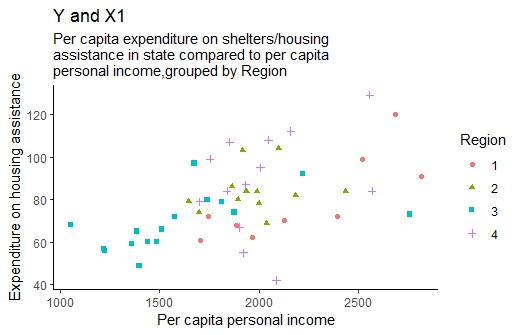
\includegraphics{YandX1byRegion}

\end{itemize}



\end{document}
